\chapter{\textsc{Solas}, A 3-D Laser Ray Trace and Cross-Beam Energy Transfer Model} \label{chap:SOLAS}



This chapter will describe the \textsc{Solas} code, a 3-D Laser ray tracing module implemented in the \ac{Rad-MHD} code \textsc{Chimera}.
The chapter begins with a discussion of why ray tracing is frequently used to model `long-pulse' lasers for \ac{HEDP} experiments and why the standard framework is inadequate to model \ac{LPIs}.
It will then go on to describe the ray-trajectory solver, electric-field reconstruction and \ac{CBET} components of the model in detail.
Discussion of the validity of the model components will be included.
The numerical methods will also be presented alongside an extensive set validation problems to verify the implementation.


%###############################################################################################################################
%###############################################################################################################################
%###############################################################################################################################
\section{Ray Tracing for Hydrodynamic Simulations of Fusion Plasmas}

Nanosecond length (`long-pulse') lasers are often used as an external energy source in the field of \ac{HEDP}, for example in laboratory-astrophysics experiments \cite{tzeferacos_laboratory_2018,fiuza_electron_2020,meinecke_strong_2022}, equation of state studies \cite{kritcher_measurement_2020} or \ac{ICF} implosions.
Experimental design and analysis for these experiments must often be supported with fluid \ac{Rad-MHD} simulations.
The laser must therefore be described in these codes by a theoretical framework that is both valid to the problem and computationally tractable.
The physical processes by which lasers interact with plasma is a result of microscopic couplings between the laser field and particles or plasma waves.
The detailed microphysics of these interactions are often studied using \ac{PiC} codes or wave-based solvers, typically for scales and durations of tens of micrometres and hundreds of picoseconds.
Coupling these tools directly to multidimensional hydrodynamic simulations, which are often used for millimetre and nanosecond scales, would usually be computationally intractable.

The \ac{GO} assumptions are often widely applicable for \ac{HEDP} laser-plasma interactions (validity discussed in detail for \ac{ICF} plasmas in section \ref{sec:model_appliciability}) and therefore ray-tracing offers a computationally tractable approach to modelling lasers in these experiments.
By assuming static hydrodynamic profiles (which is normally valid for the propagation time of light through the computational domain) a laser beam can be discretized into a bundle of rays and the ray equations can then be integrated along their path to solve for the trajectory of the light, assuming that refraction dominates over diffraction.
A discrete amount of power can also be given to each ray.
If there is a suitable model for the power-absorption rate, this can also be integrated along the ray to provide an energy source for the plasma.
In many laser-driven \ac{HEDP} experiments, frequency-doubled or -tripled lasers and long scale-length plasmas mean that \ac{IB} is the dominant deposition process.
There are well established models for \ac{IB} that are suitable for implementation in ray-tracing codes, because they only require knowledge of the local plasma conditions, which are easily accessible via interpolation from the hydrodynamic grid to rays.
The combination of the ray equations and \ac{IB} deposition therefore is the basis for the vast majority of laser-modules coupled to hydrodynamic codes.

In laser-driven \ac{ICF} experiments however, another class of interaction, \ac{LPIs} are vitally important to the energetics of the implosion.
For example \ac{CBET} leads to a zeroth-order correction to the energy deposited in direct-drive experiments at the OMEGA laser facility, reducing coupled power late in the implosion by $\sim 50\%$.
They cannot be included in the simple framework described above because they are non-linear\footnote{Non-linear in this context means that the interaction involves the interaction of multiple light and plasma waves.} and rely on knowledge of the electric field or intensity of the light.
Implementation in a tracing code therefore necessitates a method by which the separate light waves can `talk' to each other.
For example, the \ac{CBET} code described in this chapter stores information for separate components of laser beams on a common grid which can then interact via the `pump-depletion iterations', described in section \ref{sec:pump_dep_iters}.
Additionally, the knowledge of electric field or intensity is problematic because this is not an attribute which standard \ac{GO} rays posses.
Heuristically, rays have an associated power, so an area is required to obtain an intensity.
The evolution of a portion of the beam front's area is governed by a first order expansion of the Helmholtz equation, rather than the zeroth order expansion which is most commonly used in ray-tracing packages for hydrodynamic codes.
The first order expansion introduces an equation for the ray amplitude which can be solved in a variety of ways and used to obtain the electric field of the light.
Section \ref{sec:SOLAS_field_reconstruc} describes the approach taken to solving for the amplitude of the rays in \textsc{Solas}, which is to track the area of a triangle\footnote{For a 2D ray trace, a pair of rays is used rather than a triangle.} of rays around a zeroth order \ac{GO} ray.

For direct-drive \ac{ICF} simulations, it is also desirable to have a 3D ray trace, where rays travel and refract in 3 dimensions.
In some computational direct-drive studies, particularly in 1D hydrodynamic simulations, simplified laser models are employed in which rays travel radially toward the target.
This simplification is can lead to significant deviations from reality, as it neglects any refractive losses, which can be significant late in the implosion as the target converges.
It also leads to deposition occurring further in radially compared to a true 3D ray trace, leading to an overestimation of the drive.
The growth of \ac{LPIs} also depends on vector summations of light and plasma wavevectors, so a 3D ray trace is necessary when modelling these effects.
Predictive direct-drive simulations therefore necessitate a fully 3D ray-trace, even when coupled to 1D hydrodynamics.


%###############################################################################################################################
%###############################################################################################################################
%###############################################################################################################################
\section{Existing Cross-Beam Energy Transfer Models}

There are a variety of existing computational tools used to model \ac{CBET} for \ac{ICF} conditions, which are used to study the interaction from first principles, reduced models to investigate the effect of \ac{CBET} when coupled to hydrodynamics or validation tools to test the implementation of these reduced models.
A non-exhaustive list will be presented here of existing codes, provided mainly as context for the work presented in this chapter.

%################################################################################
%################################################################################
\subsection{Ray Based Models}

The most common tool to study the coupling of \ac{CBET} effects into hydrodynamics are reduced ray-based models which use the linear gain theory of \ac{SBS}, outlined in section\ref{sec:SBS_linear_gain}.
There are a variety of different codes used to simulate this.
The main difference between the models is the way that the electric field or intensity of the laser light is obtained.

\paragraph*{\ac{IRT}} This is an approach, implemented within the \textsc{Ifriit} code, that creates a mapping between points on an initial beam front and arbitrary locations within the plasma.
This is in contrast to \ac{FRT}, which is used in the other ray-based approaches listed below, where discrete points on the beam front are integrated forward to discrete points within the plasma.
\ac{IRT} is a very efficient approach for convex, approximately spherically symmetric plasma profiles, it can not deal well with beams that have multiple caustics\footnote{Caustics are defined and discussed in detail in section \ref{sec:SOLAS_ray_amplitude}.}, where the \ac{FRT} approach is better suited.
\textsc{Ifriit} has been coupled to the 3-D \ac{Rad-Hydro} code, \textsc{Aster} from \ac{LLE}, and prior to the development of \textsc{Solas}, \textsc{Aster}-\textsc{Ifriit} was the only code combination capable of conducting 3-D direct-drive simulations with in-line \ac{CBET}.

\begin{figure}[t!]
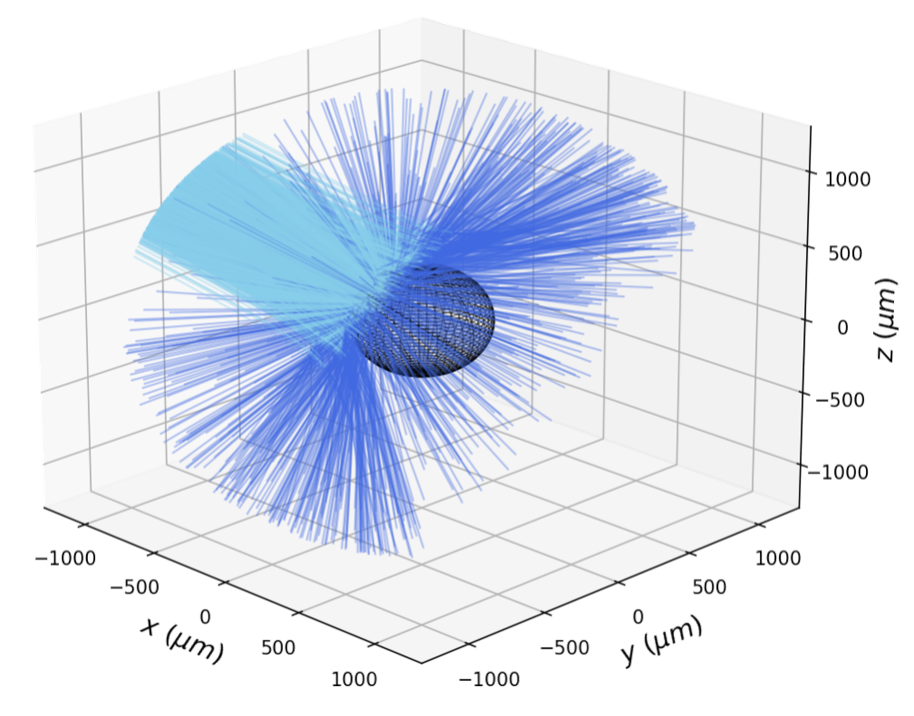
\includegraphics[width=8cm]{Numerics/Images/Reflected_Rays.png}
\centering
\caption{3D ray trajectories through a spherically symmetric, OMEGA direct-drive scale density profile.
The incident rays are plotted in cyan and the reflected rays, which spread out over a very large solid angle, are plotted in dark blue.
The critical density is represented by the black mesh.}
\label{fig:reflectedrays}
\end{figure}

\paragraph*{Ray Statistics Approach} The \textsc{Lasnex}, \textsc{Troll} and \textsc{Draco} codes, developed at \ac{LLNL}, \ac{CEA} and \textsc{LLE} respectively, implement field-reconstruction methods which depend heavily on having many rays per computational cell.
\textsc{Lasnex} and \textsc{Troll}, used mainly for indirect-drive hohlraum simulations, obtains the intensity of light by first propagating rays through the mesh and obtaining the deposited power in each grid cell.
The intensity is then obtained from the power in each cell using electromagnetic energy conservation.
Obtaining the intensity from deposition means that the field cannot be reconstructed in vacuum regions where no deposition occurs.

\textsc{Draco} uses a similar approach, but the intensity is estimated by multiplying the ray power by the path length in a cell divided by the cell volume, which gives a dimensional estimate for the intensity.
Both of these approaches require a large number of rays-per cell to accurately obtain the intensity, $\mathcal{O}(10\rightarrow100)$.
For direct-drive simulations this is extremely computationally expensive, because backscatter \ac{CBET} dominates over sidescatter, therefore the reflected field of each beam must be resolved, and each beam spreads out over a large solid angle after reflecting off a convex density profile, as is demonstrated in figure \ref{fig:reflectedrays}.
This means that orders of magnitude more rays are required than for approaches which can use a single ray per cell.

Another drawback of both of these approaches is that caustics of beams (regions where the amplitude of rays diverge) are not identifiable, and therefore fields cannot be capped to physically accurate, diffraction-limited values.
If a significant amount of \ac{CBET} occurs at caustics, such as in direct-drive \ac{ICF}, then erroneous global multipliers to \ac{CBET} gains must be applied which are effectively free parameters that must be tuned to obtain a pre-known reduction in absorbed energy.
This means that it is difficult to trust this approach for predictive direct-drive simulations.

\paragraph*{\ac{PCGO}} In this approach, each ray has an associated Gaussian intensity profile, the width of which is integrated along the ray trajectory.
A single ray can be used per cell as each ray can have an intensity which is interpolated to the mesh, but the reconstructed field at caustics is not accurate and the width evolution is only valid for a short propagation distance.
This approach was coupled to the \textsc{Chic} 2 dimensional hydrodynamics code, but is difficult to extend to 3D as the implementation relied on interacting only rays whose centroids crossed, which does not generically occur in 3D for non-coplanar rays.

\paragraph*{Neighbouring Rays} The \textsc{BeamTracer} code obtains an area for each ray by co-tracing a triangle of neighbouring rays around it that can be converted into a ray amplitude and therefore electric field from electromagnetic energy conservation.
Integrating the amplitude along the ray trajectory means that the caustics can be identified and therefore fields in those regions capped to diffraction limited values.
Each ray also has an individual field value, and it is therefore less dependent on ray-per-cell statistics than geometric models, such as that used in the \textsc{Draco} code described above.
Section \ref{sec:SOLAS_field_reconstruc} describes the implementation of this approach into the \textsc{Chimera} 3D \ac{Rad-MHD} code, which had not previously been used coupled to hydrodynamics in multidimensional simulations.


%################################################################################
%################################################################################
\subsection{Wave Solvers}

Solving Maxwell's equations with coupling to a plasma background is a useful tool for the study of \ac{LPIs}.
The main code used in the \ac{ICF} community that uses this approach is \textsc{Lpse}, which propagates light waves through a prescribed, spatially varying density, temperature and velocity profile in 1D$\rightarrow$3D.
It then solves the nonlinear coupling of electromagnetic waves by allowing first order plasma perturbations (obtained from the ponderomotive beat pattern between light), which then feed back into the wave propagation.
The perturbative approach means that \textsc{Lpse} is limited to linear problems and the temporal and spatial resolution required to resolve the beat frequency mean that coupling to multidimensional \ac{Rad-Hydro} simulations is not feasible.
However, it is an extremely useful tool to validate implementation of \ac{CBET} models, especially in situations like scattering at laser caustics, such as the test case presented in section \ref{sec:SOLAS_CBET_caustic_test}.
It can also been used for many other important studies, such as the mitigation of \ac{LPIs} via laser bandwidth and the effect of beam smoothing techniques on the growth rate of \ac{LPIs}.

%################################################################################
%################################################################################
\subsection{\ac{PiC} Codes}

Both Ray based codes and \textsc{Lpse} are ill-suited to the study of \ac{LPIs} in the non-linear regime, where the laser intensity becomes sufficiently large that the ponderomotive imprint on the plasma can no longer be treated perturbatively.
Understanding this growth and saturation of \ac{LPIs} in this regime is particularly important for \ac{ICF} schemes with high peak intensities, such as during the ignitor spike in shock ignition pulses.
Often kinetic effects such as ion-trapping become important in non-linear saturation, where ion are trapped and then accelerated in the \ac{CBET} induced \ac{IAW}, leading to changes in the \ac{IAW} phase velocity and therefore a loss of resonance.
\ac{PiC} codes are therefore well suited to model this kinetic saturation, albeit over short timescales and in simulations that are not truly representative of direct-drive conditions, due to computational expense.
Kinetic modelling of \ac{CBET} has demonstrated that the growth of \ac{LPIs} can be a much more complex, time-dependent problem than is assumed by the linear-models used in ray-based codes, leading to larger net energy transfers.

%###############################################################################################################################
%###############################################################################################################################
%###############################################################################################################################
\section{\textsc{Solas} 3-D Laser Ray Trace}

This section will follow on from the theory section which derived the equations of ray tracing.
It shall discuss 1D ray tracing and why that can be inadequate (doing CBET properly and limited to a specific use case) and compare it to 3D.


%################################################################################
%################################################################################
\subsection{Equations of Rays and Adaptive Integration}

Also mention here why I didn't use Kaiser solution (refraction from Snell was found to create unacceptable noise in the ray amplitude estimation).
Somewhere mention that ray deposition is interpolated onto neighbouring cells using shape functions to reduce noise.
Talk about how additional quantities are integrated along ray trajectory which are described in CBET section.
However, the derivatives of these other things are assumed to be constant over a single laser step and therefore are not included in the adaptive integration.

Talk about how we use adaptive RK4 to integrate rays.
Mention that adaptive solvers allow large steps in flat regions and accurately resolve the turning points.

%##################################################
\subsubsection{Ray Solver Validation}

Quadratic trough, cylindrical helix and blast wave tests

\paragraph*{Quadratic trough}
Basic test of ray solver.

\paragraph*{Cylindrical Helix}
Test of refraction in non Cartesian coordinates and also of refraction in directions without gridding.

\paragraph*{Blast wave}
Test of inverse Bremmstrahlung absorption.

%################################################################################
%################################################################################
\subsection{Ray Initialisation}

Give details on random sampling, uniform and invers-projection methods explaining their relative strengths and weaknesses.

%################################################################################
%################################################################################
\subsection{\textsc{Solas} Mesh Structure}

Talk about the parallelisation method in \textsc{Chimera} (domain based MPI) and why a good hydro domain decomposition is not good for laser load-balancing.
Mention that for direct-drive, (which drove most design philosophy for the model), laser uniformly illuminate the surface, so rays are uniformly distributed across sphere.
Therefore, Ideal domain decomposition for ray trace has processors which each cover an equal area on the surface of a sphere.
Therefore split the grid solid-angularly, so that even for 1D LDD problems, can load balance across sphere.

\subsubsection{Semi-Structured Eulerian Grid with Combined Cells}

Mention that also for 3D Eulerian spherical meshes near the poles, cell volumes go to zero.
At a minimum to estimate laser quantities within a cell, the requirement for total number of rays is therefore dictated by the polar region.
Equivalently for a given number of rays, noise will be much worse at the poles.
Therefore a novel `semi-structured' grid was designed to circumvent this issue without giving up the advantages of an Eulerian grid (ease of implementation and interpolation between grids).
Cells are combined in phi and theta to have the same dphi and dtheta as the equatorial cells on the grid, giving a roughly equal area on each raidla surface.

Also mention how cells are combined in r adaptively, which gives improved resolution in the vicinity of the caustic, where deposition, CBET and refraction are singificant.
Note however that resolution is limited to the hydrodynamic resolution and the laser grid is not entirely separate.
This does make interpolation between grids easier though.

%###############################################################################################################################
%###############################################################################################################################
%###############################################################################################################################
\section{Ray Based Field Reconstruction and Ray Sheets}
\label{sec:SOLAS_field_reconstruc}

Say that we want to find the field to get CBET.
For rays this means solving the transport equation to get ray amplitude and then using amplitude to get field.
Talk about the concept of ray amplitude and how it can be related to an area of adjacent rays.

%################################################################################
%################################################################################
\subsection{Amplitude Estimate from Neighbour Rays}
\label{sec:SOLAS_ray_amplitude}

Go into detail about how the area is obtained from neighbour rays.
Talk about the concept of sheets and caustics as divergence of amplitude.
Also talk about `Interpolation' from rays to cells and vice versa.

%################################################################################
%################################################################################
\subsection{Caustic Field Capping}
Say that since amplitude diverges in the caustic region, necessary to cap it.
In reality diffraction would limit the field in this region, but standard geometric optics rays can't model diffraction.
Therefore typical approach which we follow is to limit the reconstructed field to a sensible, diffraciton-limited value.

%##################################################
\subsubsection{Field Limiter Approach}
Say that this is the approach used throughout the thesis apart from in some validation problems where it is labelled.
Caps the field to the maximum of a Airy function (ray going up linear density profile).

%##################################################
\subsubsection{Etalon Integral}
This is an improvement which basically allows for deviations from linearity.
This is not used normally, other than when cell size << wavelength, because it needs knowledge of the other sheet from the beam which is present in caustic region.
Could be implemented using linear interpolation.
However, typically we don't have sufficient angular resolution in combined cell grid (at least for 1D hydro) to reliably interpolate sheet to sheet via this grid.
It is generally observed however that the field limiter approach is sufficient.

%################################################################################
%################################################################################
\subsection{Field Reconstruction Validation}
Using Russ' paper with lovely test comparisons to \textsc{Lpse}.
Define the electron density profile here.

%##################################################
\subsubsection{1D Reflected Beam}
Just a simple test of field capping compared to an analytic problem, without refraction.

%##################################################
\subsubsection{2D Reflected Beam}
Same as above, but now for non-normally incident rays, accounting for refraction.
Show test results in both Cartesian and Cylindrical.


%###############################################################################################################################
%###############################################################################################################################
%###############################################################################################################################
\section{Ray Based CBET Model}

Explain that ray based CBET uses the linear gain discussed in theory section.
Say that since this assumes homogineity, effectively applies to small ray steps, which is typically well satisfied.
Also say that this homogeneity within a computational cell and nearest neighbour interpolation of field means that it is not necessary to adaptively integrate the CBET gain.

%################################################################################
%################################################################################
\subsection{Power Change of Rays due to CBET}

Describe how ray energy changes due to CBET from linear gain models (either fluid or kinetic).
Say how when including with inv brem, the deposited power and CBET change must be got carefully (i.e. Marozas paper).

%##################################################
\subsubsection{Fluid CBET Gain}

Breifly discuss the fluid CBET gain and explain why it is easier to use for code validation.

%##################################################
\subsubsection{Kinetic CBET Gain}

Breifly discuss the kinetic CBET gain and why it is better for predictive simulations.

%################################################################################
%################################################################################
\subsection{Dynamic memory structure for storing Fields and CBET Gains}

Give the scaling of storing fields and gains for every beam.
Say that therefore a dynamic memory structure is used which only stores the fields and gain in cells where they are present.
Also state that although the ray trace module must be done in double to numerical errors (e.g. omega differences in resonance and difference between rays), gain is stored as a single which greatly reduces cost.
Give an estimate for how much this reduces the overall memory requirements.

%################################################################################
%################################################################################
\subsection{Doppler Shift of Frequency}

Mention time dependant refractive index results in a frequency shift of light.
This is small, however it is significant to include in CBET models as it can shift the resonance.

%################################################################################
%################################################################################
\subsection{Caustic Gain Truncation}

Say that because nearest neighbour interpolation of the fields is used, there exists unphyscial interaction regions where a cell has a field but ray hasn't passed through that portion of the cell.
This problem becomes particularly bad at ray turning points, where a significant amount fo CBET occurs.
Therefore a method called `CGT' is used to effectively enhance the laser grid resolution in the vicnity of caustics.
In cells where a ray from a specific sheet experience a caustic, the field entry for that sheet is divided geometrically, assuming that the caustic is locally a plane.
If a ray from another sheet passes through the cell and is on the `unlit' side of the caustic plane, it will not experience CBET gain.
Ray steps are also limited to the caustic plane.
Other codes have shown that this approach significantly improves energy conservation.

%################################################################################
%################################################################################
\subsection{Coherent Caustic Correction and Caustic Region Identification}

Say how the field reconstruction assumption works everywhere apart from at caustics, where it underestimates the field.
Follow what Russ says in his paper about CC correction and how it significantly improves energy conservation.

%##################################################
\subsubsection{Geometric Approach to identifying the caustic region}

Other codes find caustic region by phase diff and phase interpolation.
We can't interpolate due to resolution issues.
Therefore implemented a new, geometric approach to finding the caustic region.
Talk about how location of rays is stored for each sheet, partitioned by whether they are over or under the amplitude cap.
If a cell has rays from both in a cell, then a plane is found between the two to split the cell into caustic and non-caustic.
If a cell has only capped rays then the whole thing is caustic.
When a ray from another beam passes through, CC mult is applied if in the caustic region.


%################################################################################
%################################################################################
\subsection{Energy Conservation in Ray Based CBET Models}

Talk about how energy is conserved away from caustics when converged.

%################################################################################
%################################################################################
\subsection{Pump Depletion Iterations}
\label{sec:pump_dep_iters}

Talk about why it is necessary to iterate the ray trace.
Mention that it is possible to store ray locations and avoid performing ray trace all over again, but that approach is not taken due to memory limitations.
Talk about convergence parameter.
Mention necessity of damping for complicated, many beam simulations.

%################################################################################
%################################################################################
\subsection{Model Assumptions, Applicability and Validity to ICF}
\label{sec:model_appliciability}

Discuss the key assumptions of the CBET model and whether it is valid to use for LDD and LID.

%################################################################################
%################################################################################
\subsection{Computational Efficency and Scaling}

Talk about how the CBET model is quite expensive.
Give the scaling laws from Russ' paper and explain how that means for many beams, CBET is bound to be the dominant cost in the simulation.
Also say how it shows that memory is a big consideration for CBET models as the gains and fields must be stored.

%################################################################################
%################################################################################
\subsection{\ac{CBET} Validation}
Using Russ' paper with lovely test comparisons to \textsc{Lpse}.
Define the electron density profile here.

%##################################################
\subsubsection{2D \ac{CBET} Without Caustics}
Just a simple test of field capping compared to an analytic problem, without refraction.

%##################################################
\subsubsection{2D \ac{CBET} With Caustics}
\label{sec:SOLAS_CBET_caustic_test}
Same as above, but now for non-normally incident rays, accounting for refraction.
Show test results in both Cartesian and Cylindrical.


%###############################################################################################################################
%###############################################################################################################################
%###############################################################################################################################
\section{Coupling to Hydrodynamics and Example Use}

Here present an entire explanation for the model working coupled to Hydrodynamics.

%################################################################################
%################################################################################
\subsection{Power Deposition}

Say that the deposited power is just added as an energy source to the electrons.
If running in 1D or 2D, it is integrated over other directions first.
Say that when starting from $t=0$, often use a cold-start routine, which uniformly deposits power at the critical surface of a spherical capsule.
This creates an under-dense small region in which the rays can refract and deposit energy.
This is unsatisfactory for imprint simulations, where early time imprinting is important, but that is not considered for this thesis.

%################################################################################
%################################################################################
\subsection{Time step limiter} \label{dtlaser}

Limit timstep based on the fractional electron energy change.
Don't limit timestep in cells far from critical.
This is usually the limitting timestep for `cold start' simulations initially, until deposition begins to occur in hot cells.

%################################################################################
%################################################################################
\subsection{Ray Trace Frequency}

For many beam simulations, such as direct-drive simulations, the laser operator (especially with CBET) is typically one of the more expensive parts of the code.
In the steady state of an implosion, the coronal plasma conditions don't significantly change on the global hydrodynamic timestep.
Therefore the deposition also doesn't change much meaning that previously calculated Pdep can be stored and reapplied on subsequent timesteps.
Especially for CBET simulations, this can reduce runtime by order of magnitude.
Currently the ray trace is performed every timestep up until a pre-specified `warm up' time has expired.
Then the ray trace is performed at a pre-specified frequency by the user.
Experimentation has found that for \textsc{Omega} scale simulations, increasing frequency of calculations doesn't significantly change the answer above ... .

Because LDD pulses often start with a low intensity and then ramp up, CBET gains are also often minimal until late in the implosion.
Therefore field reconstruction and CBET iterations are only performed after a specified start time, normally when the hard-sphere intensity reaches about $1\times 10^{14}$ $Wcm^{-2}$.
CBET iterations are then performed on the laser frequency.

An improved approach shall soon be implemented where laser iterations occur at $dt_{\text{laser}}$ from section \ref{dtlaser}.

%################################################################################
%################################################################################
\subsection{Computational Diagnostics}

Say that a variety of diagnostics can be output.
Qpower with and without CBET.
Geometric intensity.
Electric field (from single or all beams), optionally split into inbound and reflected components, both with and without CBET.

%################################################################################
%################################################################################
\subsection{Example use on \textsc{Omega} Shot 89224}

First briefly describe the shot, showing pulse shape and target.

%##################################################
\subsubsection{1-D Rad-Hydro, 3-D Ray-Trace with CBET Simulation}

Describe the simulation parameters used, e.g. cell resolution, flux limiter etc.
Show the absorbed power vs time and effect of CBET.
Show instantaneuos radial profiles.
Show integrated parameter comparison to \textsc{Lilac} post-shot simulation.
Describe the previous method of tuning, involving a 2D scan of flux limiter and power multipliers.
Say how it's great that the $flim_e = 0.06 \rightarrow 0.15$ and CBET combination now gives a predictive capability for \textsc{Omega} shots.

%##################################################
\subsubsection{3-D Post Process of Absorption Non-Uniformity}

Mention how the model can also be used as a postprocess.
\textsc{Chimera} can restart from 1-D data into spherically symmetric 3-D profiles.
Ray Trace and CBET can then be performed through these profiles to understand the absorption non-uniformity present due to CBET.
Note that comparison of 1-D and 3-D simulations shows that thermal conduction does a good job of smoothing angular deviations in coronal plasma conditions.
The assumption of spherically symmetric profiles for the laser is therefore deemed valid, and it is a technique typically used by post-process CBET codes.

MAYBE??
Mention how ray noise means that we can't use direct deposition.
Therefore use Pdep from field estimate, which is much cleaner.

Talk about how CBET enhances angular non-uniformity.
Show modal decomposition.


%###############################################################################################################################
%###############################################################################################################################
%###############################################################################################################################
\section{Future Model Extensions}

Say that there is even more laser/ CBET physics that is interesting and can be implemented within the raytracing framework.
Some are straightforward to implement, while others more difficult and computationally expensive.

%################################################################################
%################################################################################
\subsection{Langdon Effect on Abosprtion}

Describe Langdon from a kinetic perspective and why it reduces absorption.
Describe how you can fit it and include as a modification to ray tracing absorption if you have the field/ intensity.
Describe the magnitude of the effect for ICF like conditions.
Describe breifly how it would be implemented, say it would not be difficult.

%################################################################################
%################################################################################
\subsection{Langdon Effect on CBET}

Describe what this is.
Say that it is important for high overlapping intensities, eg hohlraum LEH.
Say that it is thought to stabilise the CBET interaction in indirect drive configurations and remove the need for artificial clamps.
Describe breifly how it would be implemented, say it would not be difficult.

%################################################################################
%################################################################################
\subsection{Polarised CBET}

Describe how ion accoustic waves are driven by beat between electric fields from light and therefore is polarisation dependent.
Say how on OMEGA, RPP smoothing means that each beam is split into 2 sub-beams with linear polarisation.
Say that these do not have a symmetry to the configuration about the sphere.
Say that this leads to mode-1 on OMEGA.
Say that you can track polarisation of rays and trace these sub-beams independently.
Would make it more expensive, but definitely feasible.

%################################################################################
%################################################################################
\subsection{Bandwidth for CBET Mitigation Studies}

Describe how bandwidth should reduce LPI growth rates.
Understanding the desired bandwidth to mitigate CBET is a key consideration for design of future laser sysytems.
Fields can be modified to include discrete wavelengths to model bandwidth.

%################################################################################
%################################################################################
\subsection{Additional LPIs}

Could look at TPD, SBS and SRS.
In theory not a difficult problem to do backscatter, but side-SRS is difficult, because additional rays would need to be launched.
This could make the model more useful to indirect-drive experiments and design of ignition scale direct-drive facilities, where SRS is thought to be important energetically due to long scale lengths.



%###############################################################################################################################
%###############################################################################################################################
%###############################################################################################################################
\section{Conclusions}

Say that the chapter has described the validity and implementation of \textsc{Solas} and validated it.
Culminated in demonstrating that the model can reproduce post-shot simulations of an \textsc{Omega} shot from the \textsc{Lilac} code which includes a CBET model.
This demonstrates that the \textsc{Chimera} code now has a predictive capability for \textsc{Omega} scale direct drive experiments, as no free parameter tuning was required.
